%/*% pdflatex -file-line-error -interaction nonstopmode %

\documentclass{article}
\usepackage{graphicx}
\graphicspath{ {./images/2.2/} }
\usepackage{amsmath}
\usepackage{amsfonts}
\usepackage{bookmark}
\usepackage{exercises}
\usepackage{amsthm}
\usepackage{yhmath}
\usepackage{placeins}
\newcommand*{\oldneg}{\mathord{\sim}}

\theoremstyle{definition}
\newtheorem{definition}{Definition}

\setlength{\parindent}{.5in}
\setlength{\parskip}{12pt}

\title{2.2 Answers}
\begin{document}
\maketitle

\section*{1}
This is a 4th degree polynomial. The type of a 4th degree polynomial is quartic. It leading coefficient is $-5$, and its constant term is $6$.

\section*{2}
The end behavior of $f(x)$ as $x\rightarrow\infty$ is what $y$ value $f(x)$ approaches as $x\rightarrow\infty$, that is, the limit of $f(x)$ in this 
direction. Similarly, the end behavior of $f(x)$ as $x\rightarrow -\infty$ is what $y$ value $f(x)$ approaches as $x\rightarrow -\infty$, that is, 
the limit of $f(x)$ in the opposite direction.

\section*{3}
This is a polynomial function. It is a quadratic function of degree $2$, and has a leading coefficient of $-1$. Its standard form is:
\[ f(x)=-x^2+8 \]

\section*{4}
This is a polynomial function. It is a quartic function of degree $4$, and has a leading coefficient of $8$. Its standard form is:
\[ f(x)=8x^4+6x-3 \]

\section*{5}
This is a polynomial function. It is a quartic function of degree $4$, and has a leading coefficient of $\pi $. Its standard form is:
\[ g(x)=\pi x^4+\sqrt{6} \]

\section*{6}
This function is not a polynomial function, as one of the exponents, $-2$, is not a whole number.

\section*{7}
This is a polynomial function. It is a cubic function of degree $3$. Its leading coefficient is $-\frac{5}{2}$. Its standard form is:
\[ h(x)=-\frac{5}{2}x^3+3x-10 \]

\section*{8}
This is not a polynomial function, as one of the exponenets, $-1$ (from $\frac{2}{x}$) is not a whole number. 

\section*{13}
\[
\begin{array}{rl}
	& h(x)=x+\frac{1}{2}x^4-\frac{3}{4}x^3+10;x=-4 \\
=	& -4+\frac{1}{2}(-4)^4-\frac{3}{4}(-4)^3+10 \\
=	& -4+128+48+10 \\
=	& 182
\end{array}
\]

\section*{14}
\[
\begin{array}{rl}
	& g(x)=4x^5+6x^3+x^2-10x+5;x=-2 \\
=	& 4(-2)^5+6(-2)^3+(-2)^2-10(-2)+5 \\
=	& -128-48+4+20+5 \\
=	& -147
\end{array}
\]

\section*{21}
$h(x)=-7x^3+11x^2+4x$;$x=3$
\begin{table}[h!]
        \begin{center}
                \begin{tabular}{l|c|c|c|r}
                        $3$ & $-7$ & $11$ & $4$ & $0$ \\
                        \hline
                        $$ & $$ & $-21$ & $-30$ & $-78$ \\
                        \hline
                        $$ & $-7$ & $-10$ & $-26$ & $-78$
                \end{tabular}
        \end{center}
\end{table}

\section*{22}
$f(x)=x^4+3x-20$;$x=4$
\begin{table}[h!]
        \begin{center}
                \begin{tabular}{l|c|c|c|c|r}
                        $4$ & $1$ & $0$ & $0$ & $3$ & $-20$ \\
                        \hline
                        $$ & $$ & $4$ & $16$ & $64$ & $268$ \\
                        \hline
                        $$ & $1$ & $4$ & $16$ & $67$ & $248$
                \end{tabular}
        \end{center}
\end{table}

\section*{23}
The error here is that the term for $x^3$ was left out of the table. Instead, we should do the following:
\begin{table}[h!]
        \begin{center}
                \begin{tabular}{l|c|c|c|c|r}
                        $-2$ & $-4$ & $0$ & $9$ & $-21$ & $7$ \\
                        \hline
                        $$ & $$ & $8$ & $-16$ & $14$ & $14$ \\
			\hline
			$$ & $-4$ & $8$ & $-7$ & $-7$ & $21$
                \end{tabular}
        \end{center}
\end{table}

\section*{24}
A

\section*{25}
The degree is even and the leading coefficient is positive.

\section*{26}
The degree is odd and the leading coefficient is negative.

\section*{27}
The deegree is even and the leading coefficient is negative.

\section*{28}
$f(x)\rightarrow +\infty$ as $x\rightarrow -\infty$ and $f(x)\rightarrow +\infty$ as $x\rightarrow +\infty$

\section*{29}
$f(x)\rightarrow -\infty$ as $x\rightarrow -\infty$ and $f(x)\rightarrow -\infty$ as $x\rightarrow +\infty$

\section*{30}
$f(x)\rightarrow -\infty$ as $x\rightarrow +\infty$ and $f(x)\rightarrow +\infty$ as $x\rightarrow -\infty$ 

\section*{31}
$f(x)\rightarrow +\infty$ as $x\rightarrow +\infty$ and $f(x)\rightarrow -\infty$ as $x\rightarrow -\infty$

\section*{32}
$f(x)\rightarrow +\infty$ as $x\rightarrow +\infty$ and $f(x)\rightarrow +\infty$ as $x\rightarrow -\infty$

\section*{33}
$f(x)\rightarrow -\infty$ as $x\rightarrow +\infty$ and $f(x)\rightarrow +\infty$ as $x\rightarrow -\infty$

\section*{34}
$f(x)\rightarrow +\infty$ as $x\rightarrow +\infty$ and $f(x)\rightarrow -\infty$ as $x\rightarrow -\infty$ 

\section*{35}
$f(x)\rightarrow +\infty$ as $x\rightarrow +\infty$ and $f(x)\rightarrow +\infty$ as $x\rightarrow -\infty$

\section*{36}
$f(x)\rightarrow -\infty$ as $x\rightarrow +\infty$ and $f(x)\rightarrow +\infty$ as $x\rightarrow -\infty$

\section*{37}
$f(x)=-5x^5$

\section*{48}
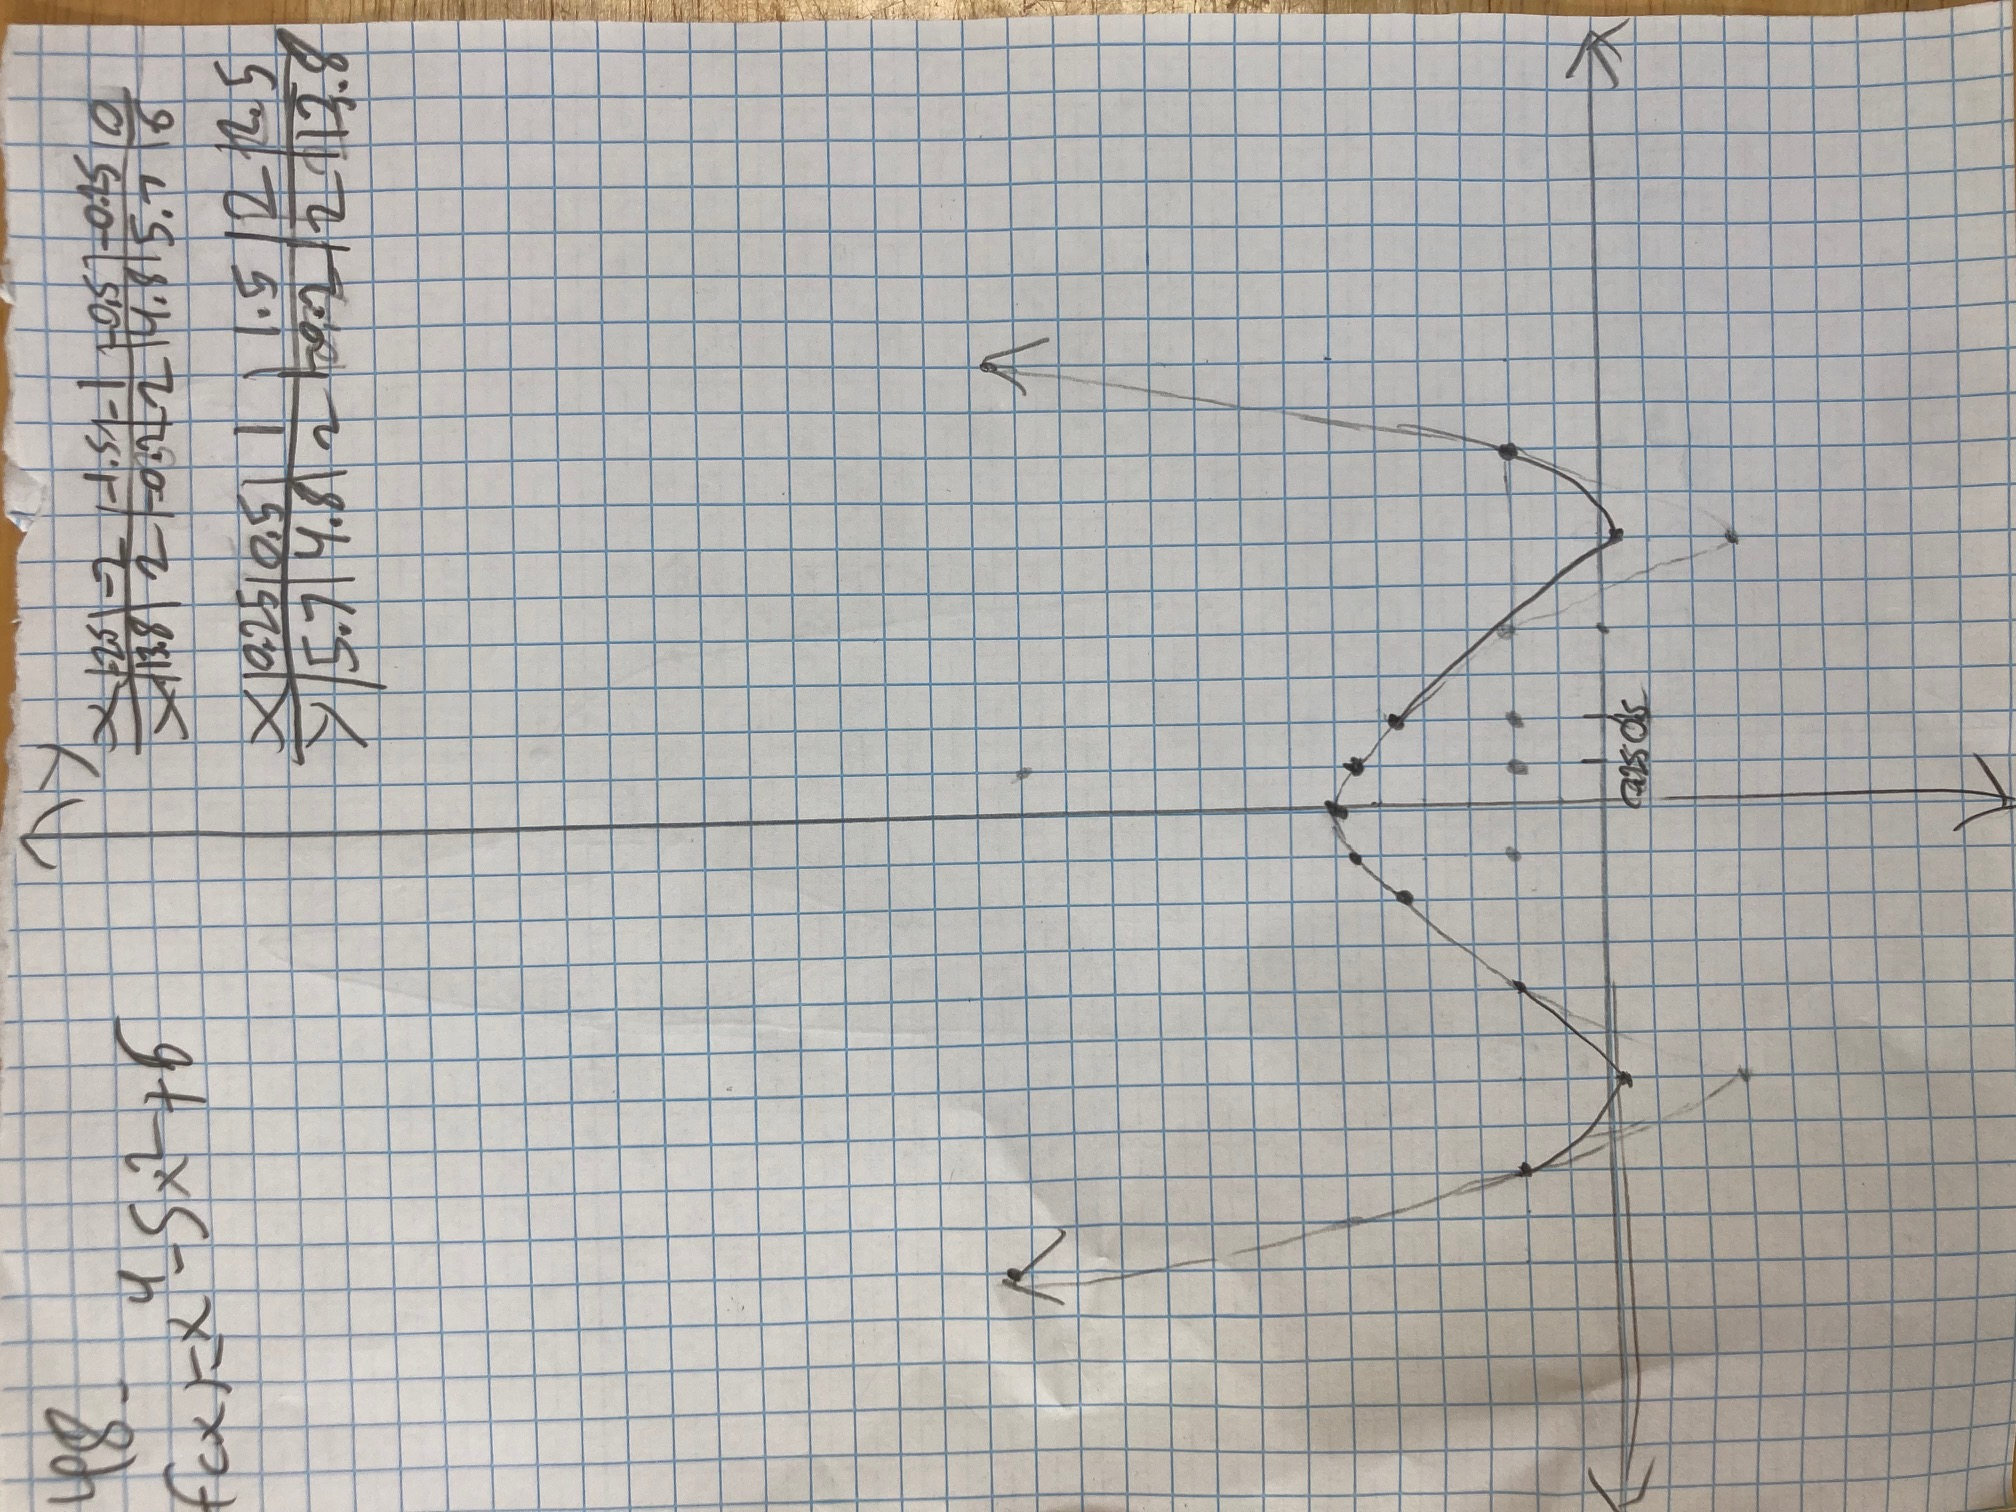
\includegraphics[width = 4in, height = 4in, angle = -90]{48picture}

\section*{49}
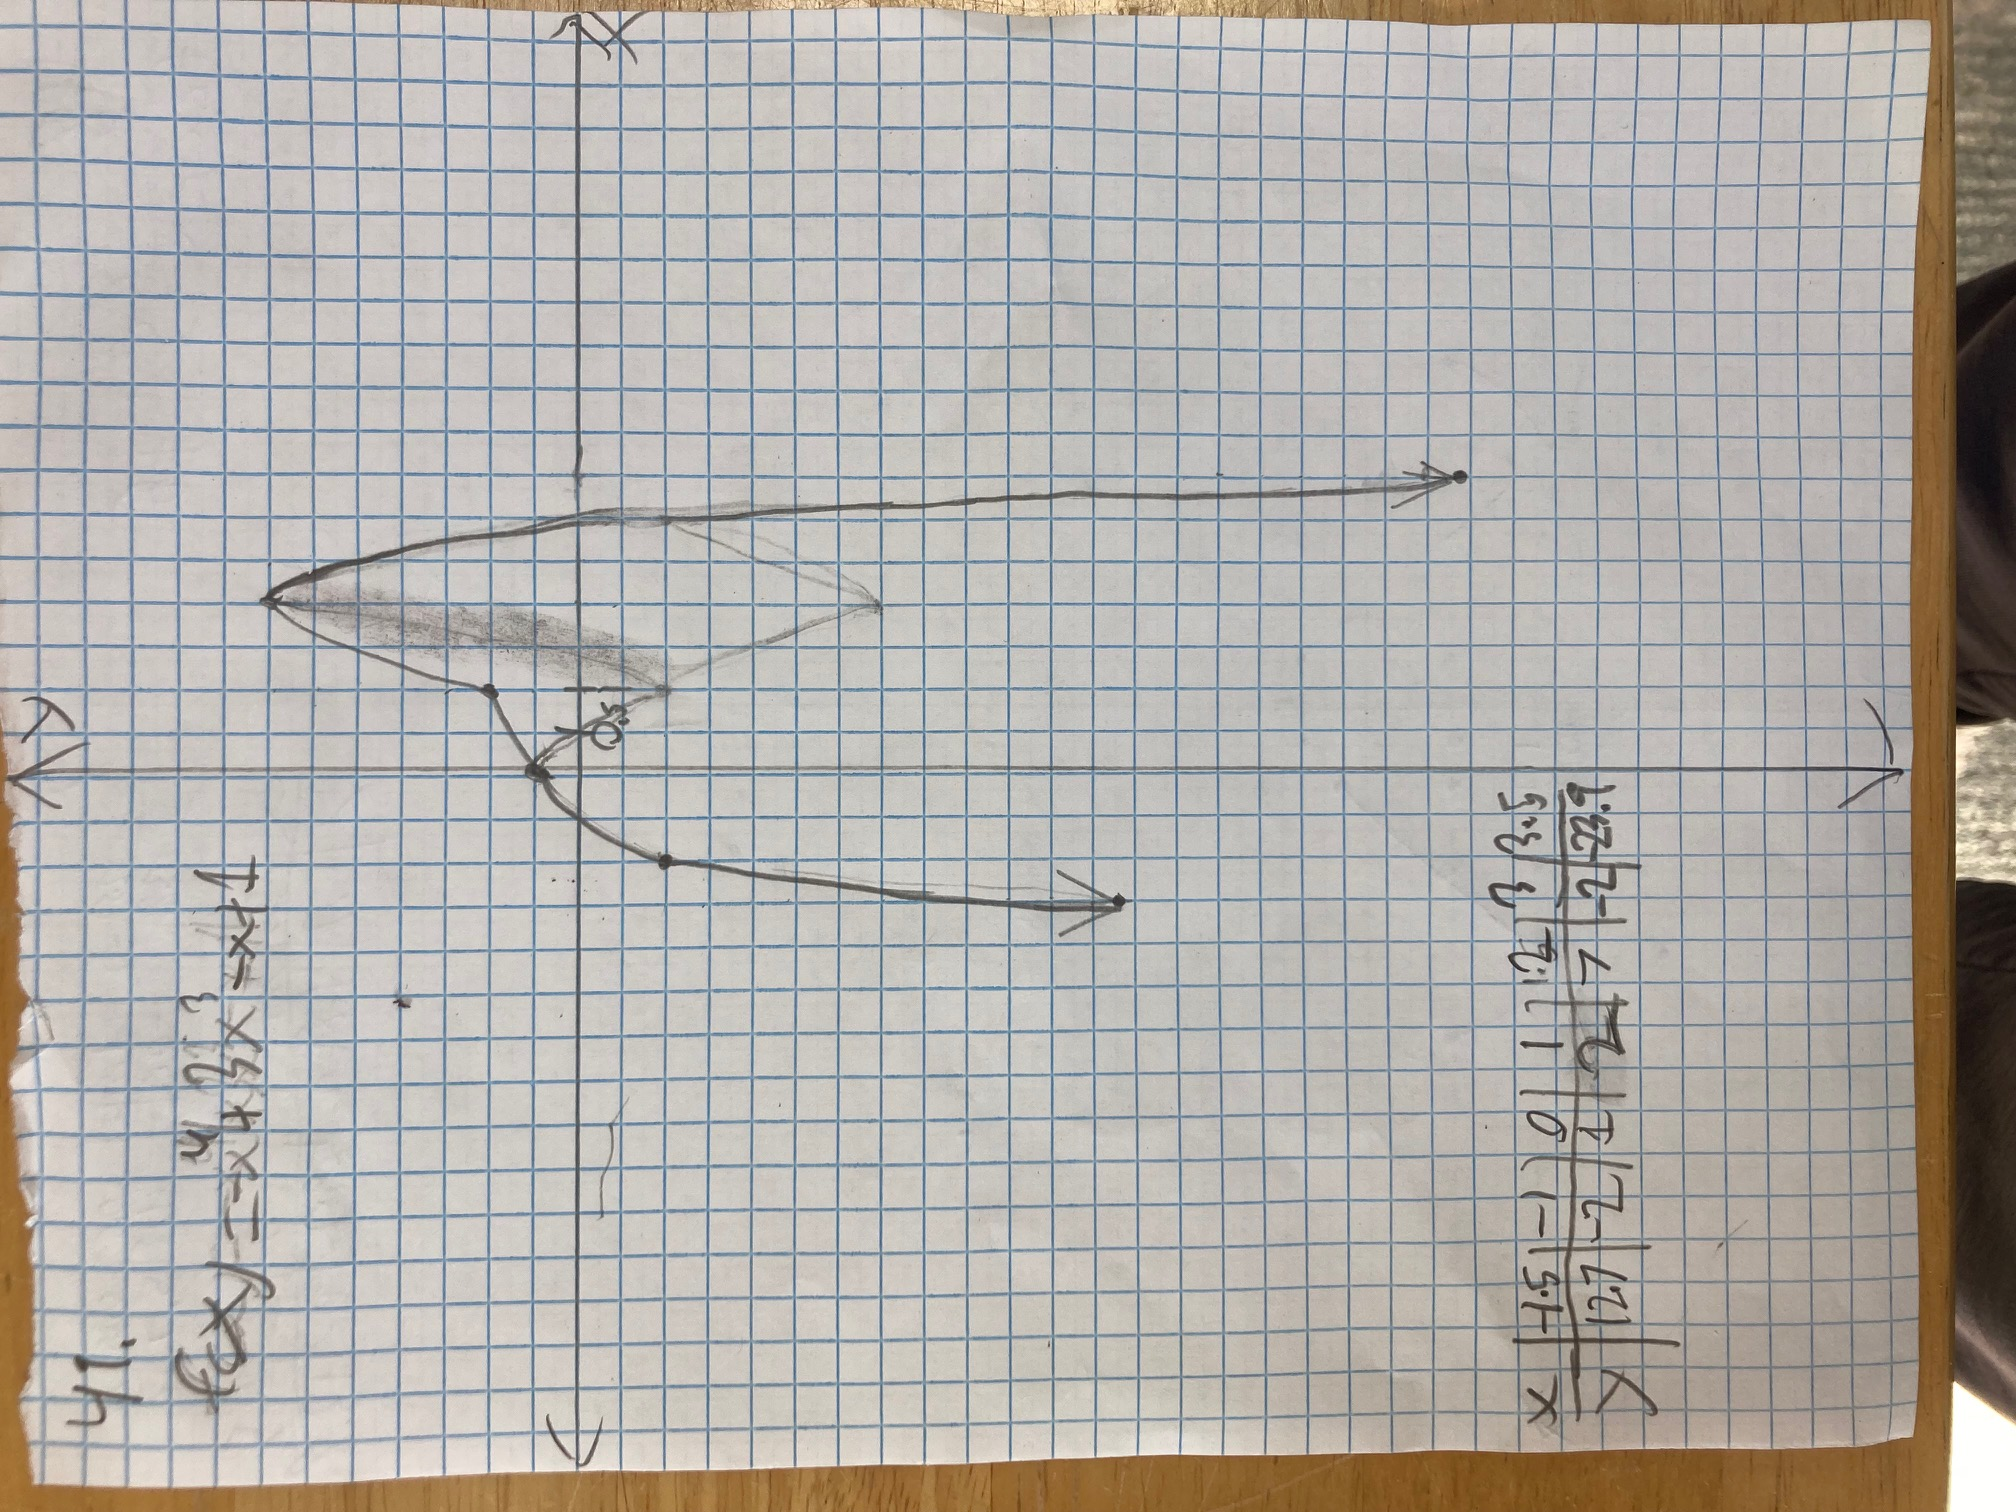
\includegraphics[width = 4in, height = 4in, angle = -90]{49picture}

\section*{50}
B

\section*{51}
$-f(x)$ will have the opposite sign as $f(x)$. We are given that $f(x)\rightarrow +\infty$ as $x\rightarrow -\infty$ meaning 
$g(x)=-f(x)\rightarrow -\infty$ as $x\rightarrow -\infty$. Also, because $f(x)\rightarrow -\infty$ as $x\rightarrow +\infty$, 
$g(x)=-f(x)\rightarrow +\infty$ as $x\rightarrow +\infty$.

\section*{52}
(I was not sure why this table came out looking so strange)\newline
We  are given that $f$ is a cubic polynomial function with a leading coefficient of $2$ and a constant term of $-5$. This means that 
this function is of the form: $f(x)=2x^3+ax^2+bx-5$. We are given that $f(1)=0$ and $f(2)=3$, meaning we can solve the system of equations: 
\[
\begin{array}{rl}
            & 0=2(1)^3+a(1)^2+b(1)-5 \wedge 3=2(2)^3+a(2)^2+b(2)-5\\
\rightarrow & b=-a+3\textrm{ (From the first equation, solving for b)}\\
\rightarrow & 3=16+4a+2(-a+3)-5 \\
\rightarrow & 3=11+4a-2a+6 \\
\rightarrow & 3=2a+17 \\
\rightarrow & 2a=-14 \\
\rightarrow & a=-7 \\
\rightarrow & b=-(-7)+3=10\textrm{ (From the second line)}
\end{array}
\]
thus meaning that $f$ is the equation $2x^3-7x^2+10x-5$, meaning $f(-5)=2(-5)^3-7(-5)^2+10(-5)-5=-480$

\section*{53}
(a): By graphing, one can see that all of the $x^n$ where $n$ is odd are symmetric with respect to the origin, and are symmetric with respect to the 
$y$-axis when $n$ is even.\newline
(b): From part (a), a noticeable pattern that can be observed is that the graph is symmetric with respect to the origin when $n$ (from $x^n$) is odd, 
and is symmetric with respect to the $y$-axis when $n$ is even. Thus, we can predict that $x^{10}$, because it is even, will be symmetric with respect to 
the $y$-axis, and $x^{11}$, because it is odd, will be symmetric with respect to the origin.\newline
(c): 
We are considering the graph of $y=x^{-n}$, which is the same as saying $y=\frac{1}{x^n}$. Suppose some point $(a,b)$ is on the graph. 
Well, consider $y=\frac{1}{(-a)^n}$ If $n$ is even, $(-a)^n$ will be positive, and will be negative if $n$ is odd. In the first case, 
where $n$ is even and $(-a)^n$ is positive, $\frac{1}{(-a)^n}=\frac{1}{a^n}=b$, meaning in this case the graph would be symmetric 
with respect to the $y$-axis. In the second case, where $n$ is odd and $(-a)^n$ is negative, $\frac{1}{(-a)^n}=\frac{1}{-(a)^n}=-\frac{1}{a^n}=-b$, 
meaning in this case the graph would be symmetric in respect to the origin. 

\section*{54}
We are given a model, so the weight of the given diamond can be found by plugging in $15$ into the model:
$w=0.0071(15)^3-0.090(15)^2+0.48(15)\approx 10.91$ meaning the diamond weights about $10.91$ carats.

\section*{55}
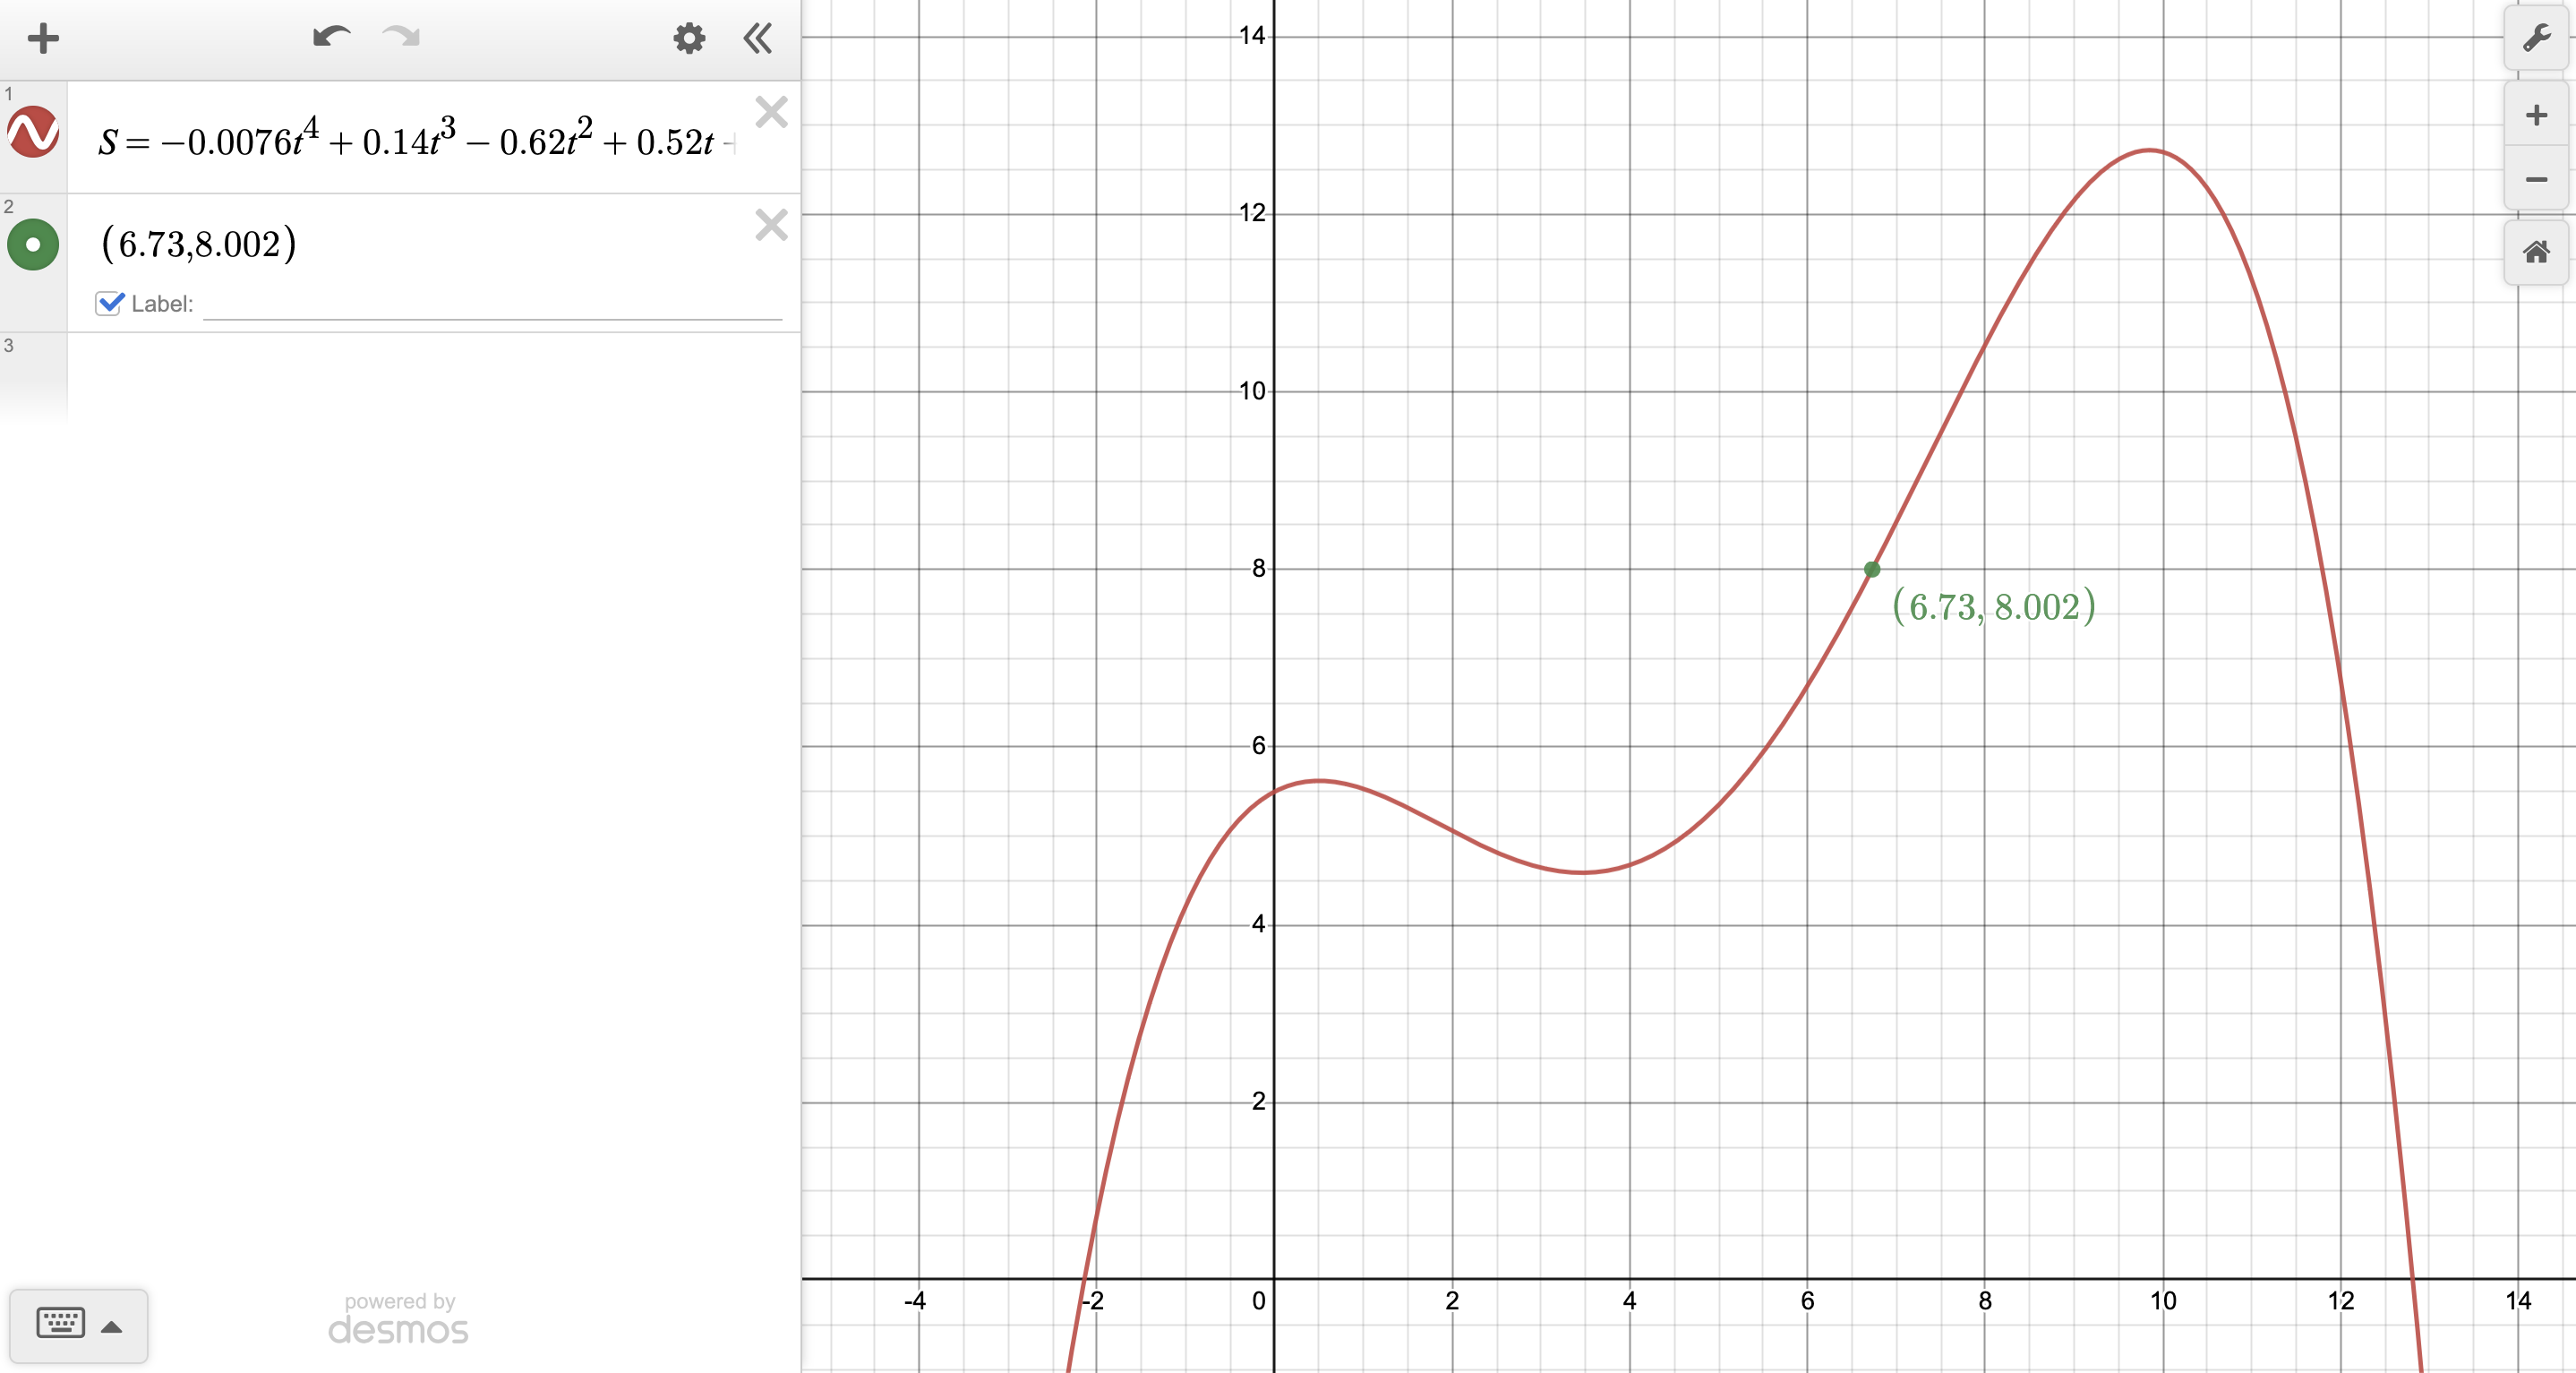
\includegraphics[width = 4in, height = 4in]{2.2picture1}
\newline From the picture, we can see that the first time there were more than $8$ million participants was approximately in $1992+6.73\approx 1998$.

\section*{56}
(I could not figure out how to make the (c) come before the graph, not after it like it is now)\newline
(a): The function is of degree $3$, and is thus a cubic function.\newline
(b):
\begin{table}[h!]
        \begin{center}
                \begin{tabular}{l|c|c|c|c|c|c|c|r}
                        $x$ & $-3$ & $-2$ & $-1$ & $0$ & $1$ & $2$ & $3$\\
                        \hline
                        $y$ & $26076$ & $23940$ & $22470$ & $21600$ & $21264$ & $21369$ & $21930$
                \end{tabular}
        \end{center}
\end{table} 
\newline (c):\newline 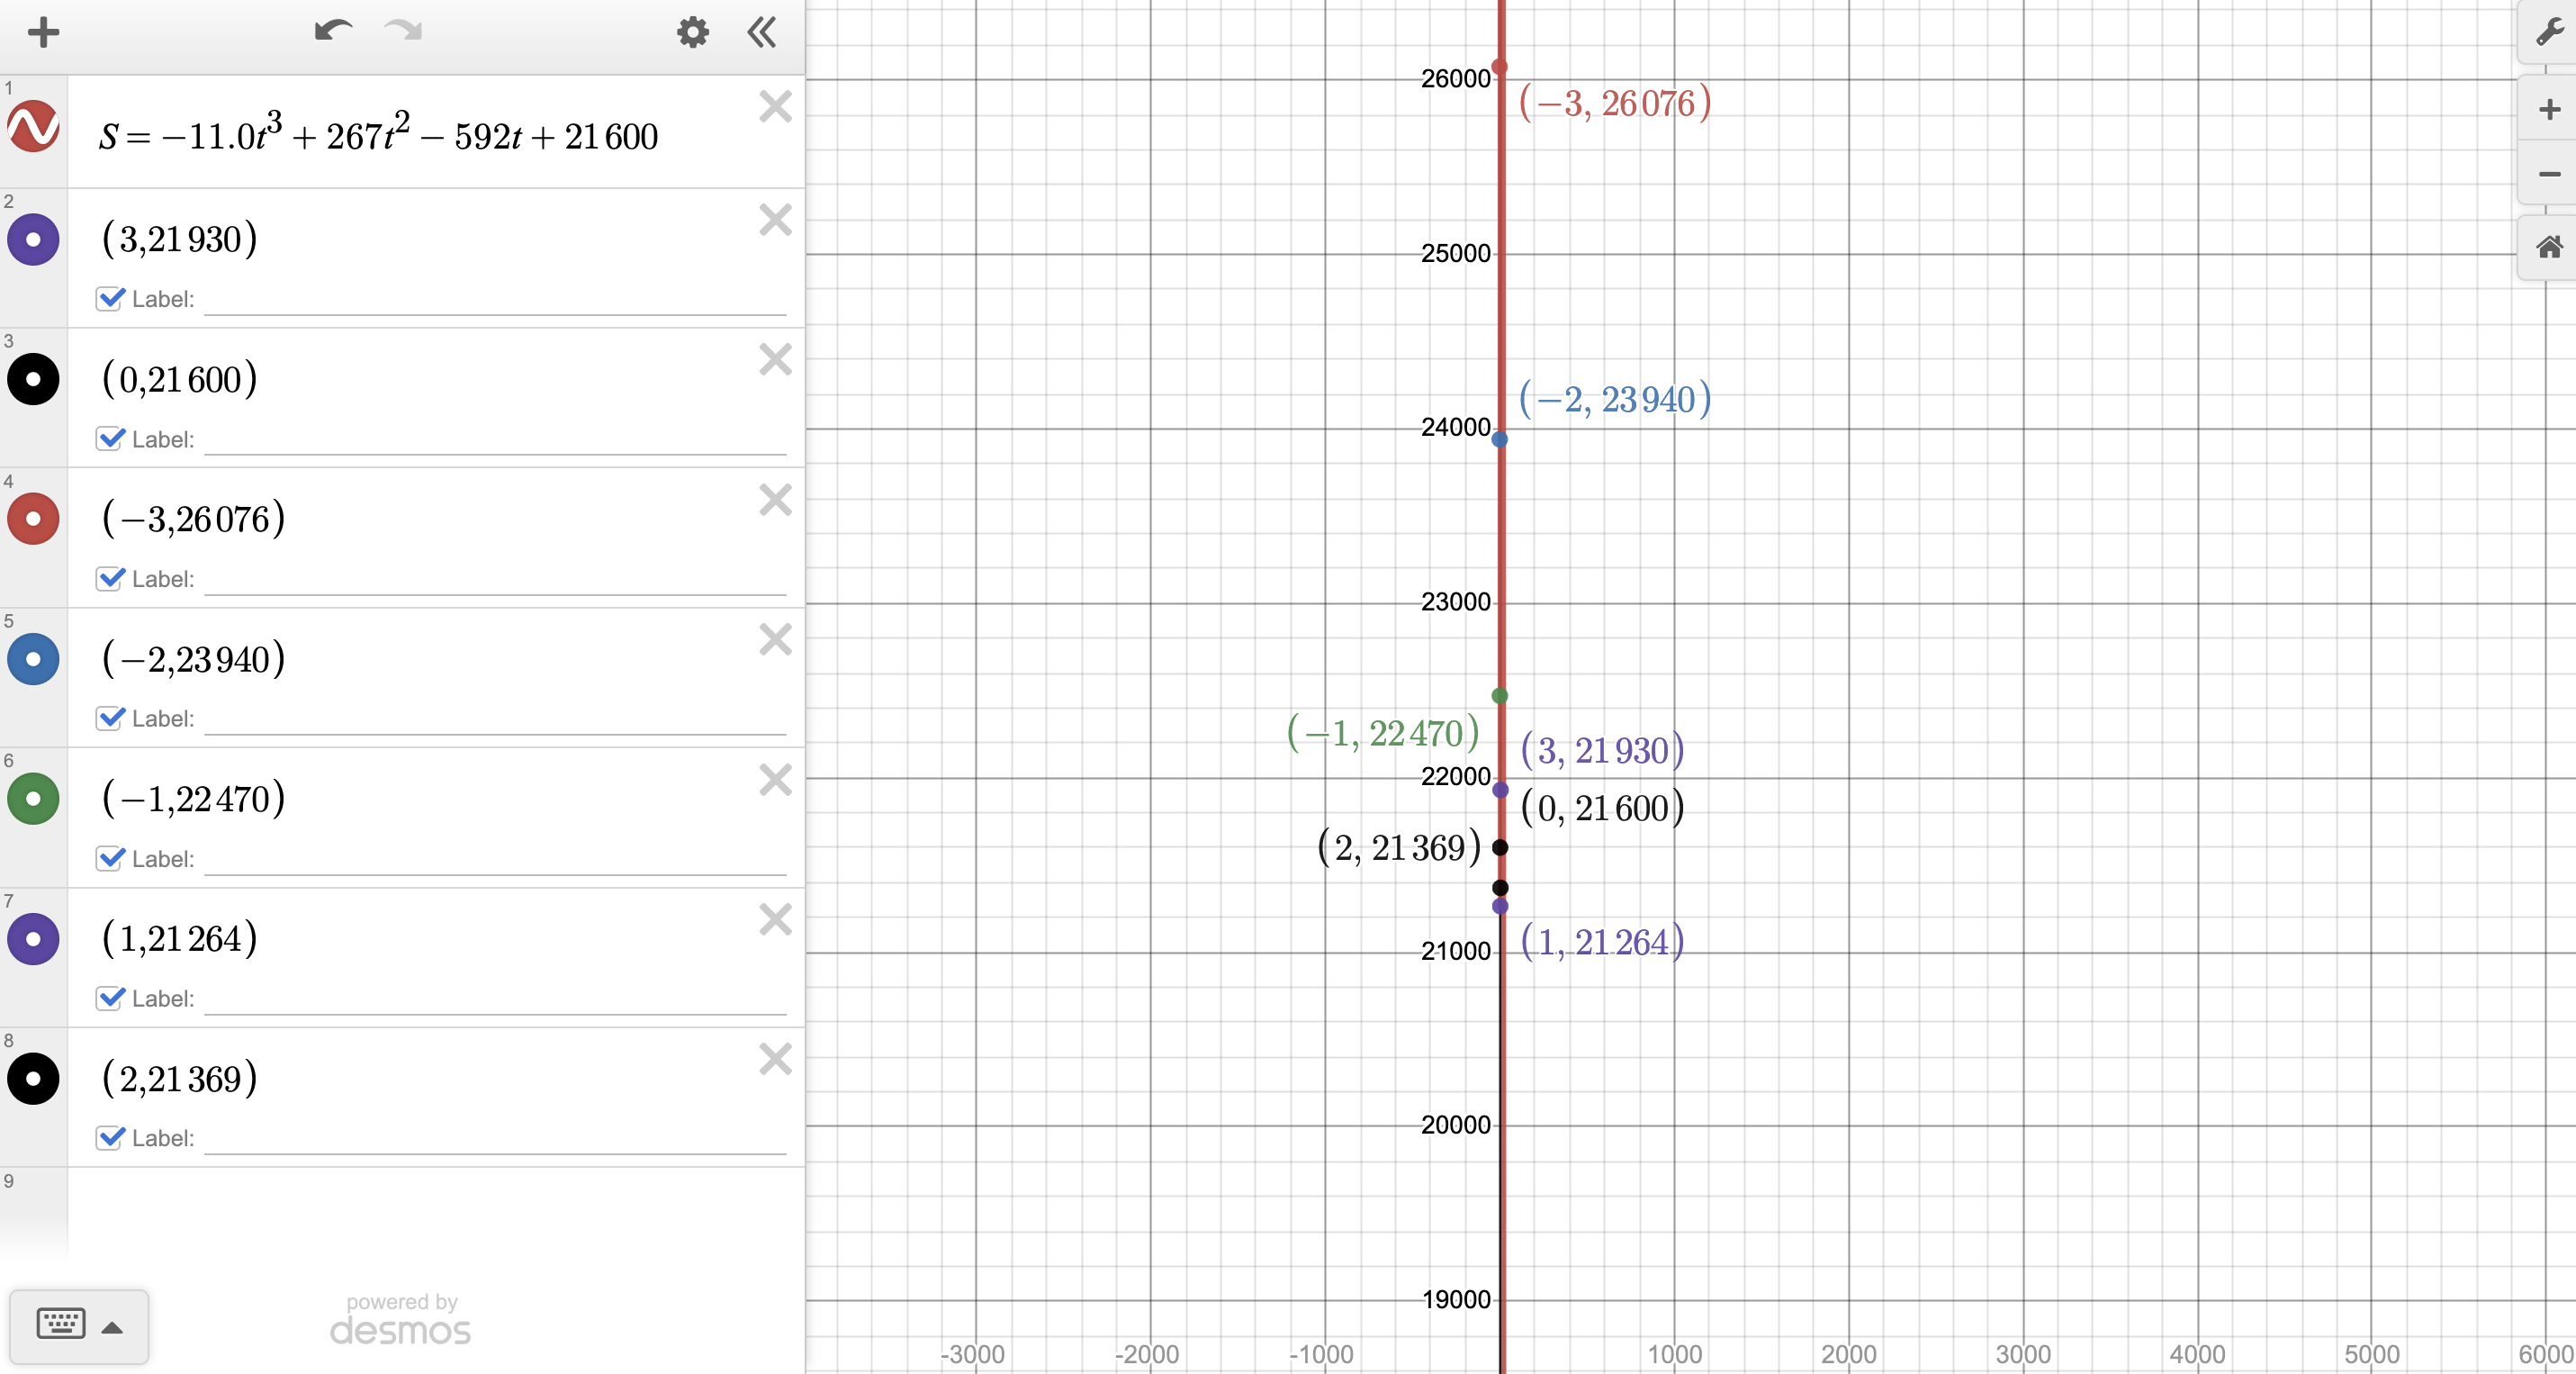
\includegraphics[width = 4in, height = 4in]{2.2picture2}

\section*{57}
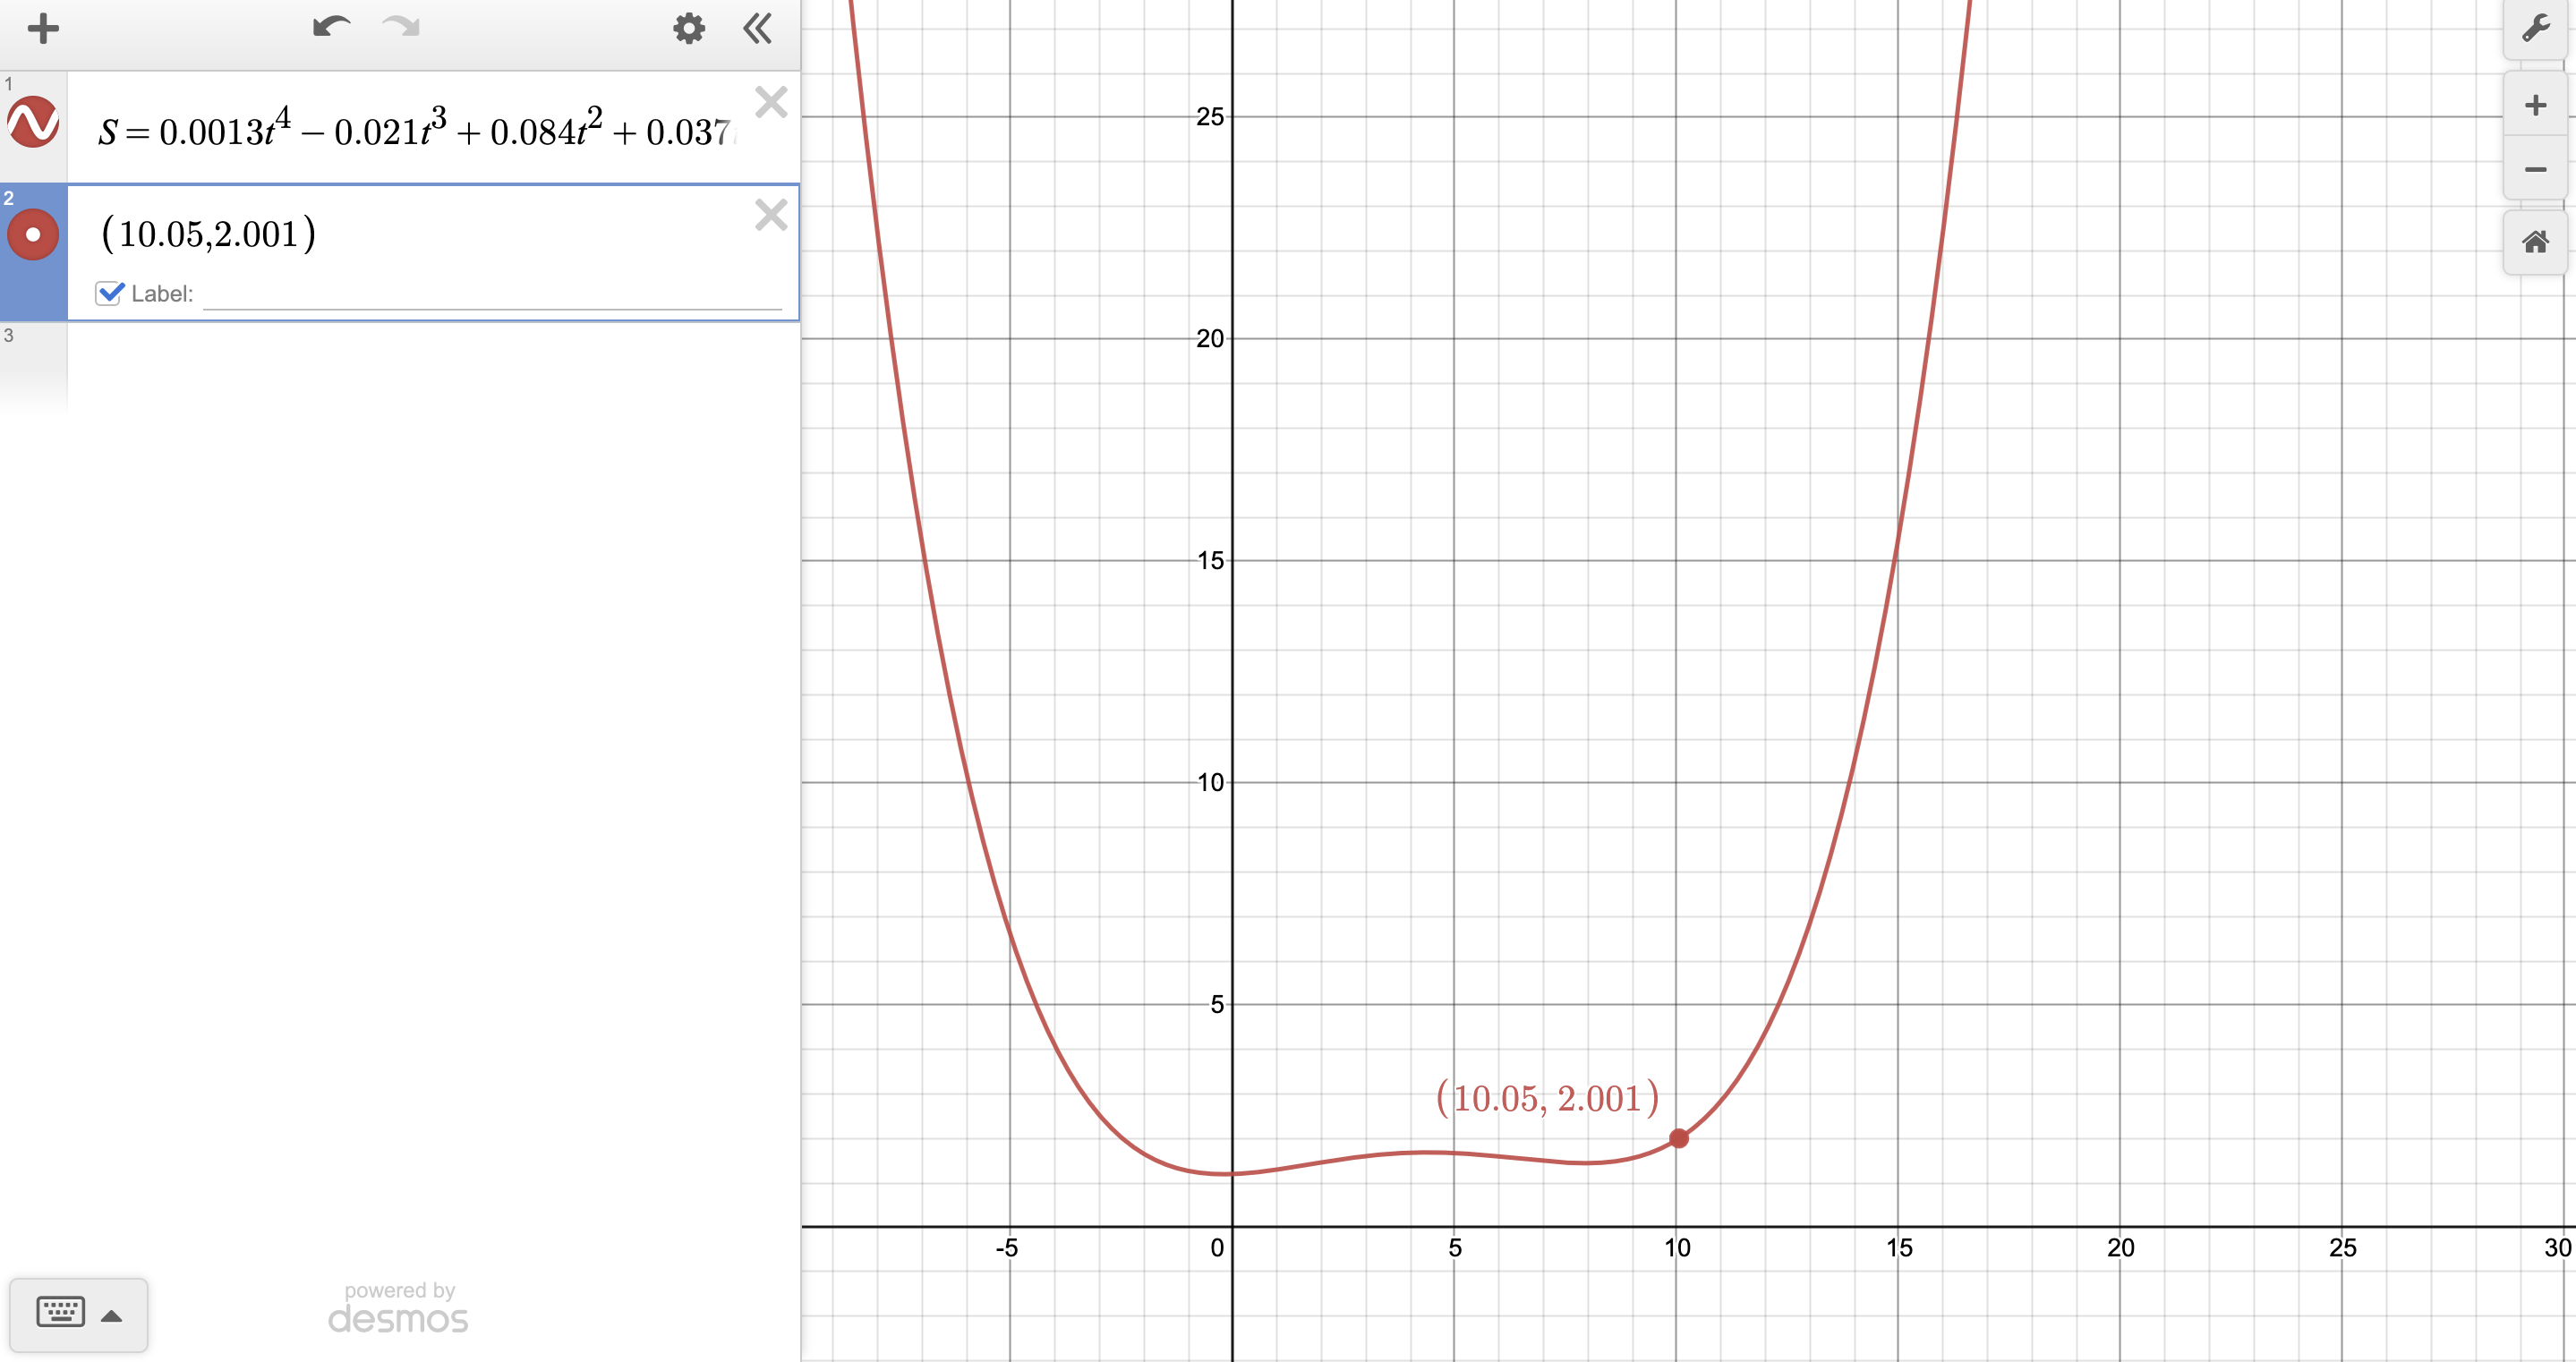
\includegraphics[width = 4in, height = 4in]{2.2picture3}
\newline From the graph, we can see that the first year where the number of snowboarding participants was greater than $2$ million was about $10$, 
meaning this year was $1992+10=2002$.

\section*{58}
(a): We are given a graph with an even degree such that the leading coefficient is positive, meaning $f(x)\rightarrow +\infty$ as $x\rightarrow -\infty$ 
and $f(x)\rightarrow +\infty$ as $x\rightarrow +\infty$.\newline
(b):\newline 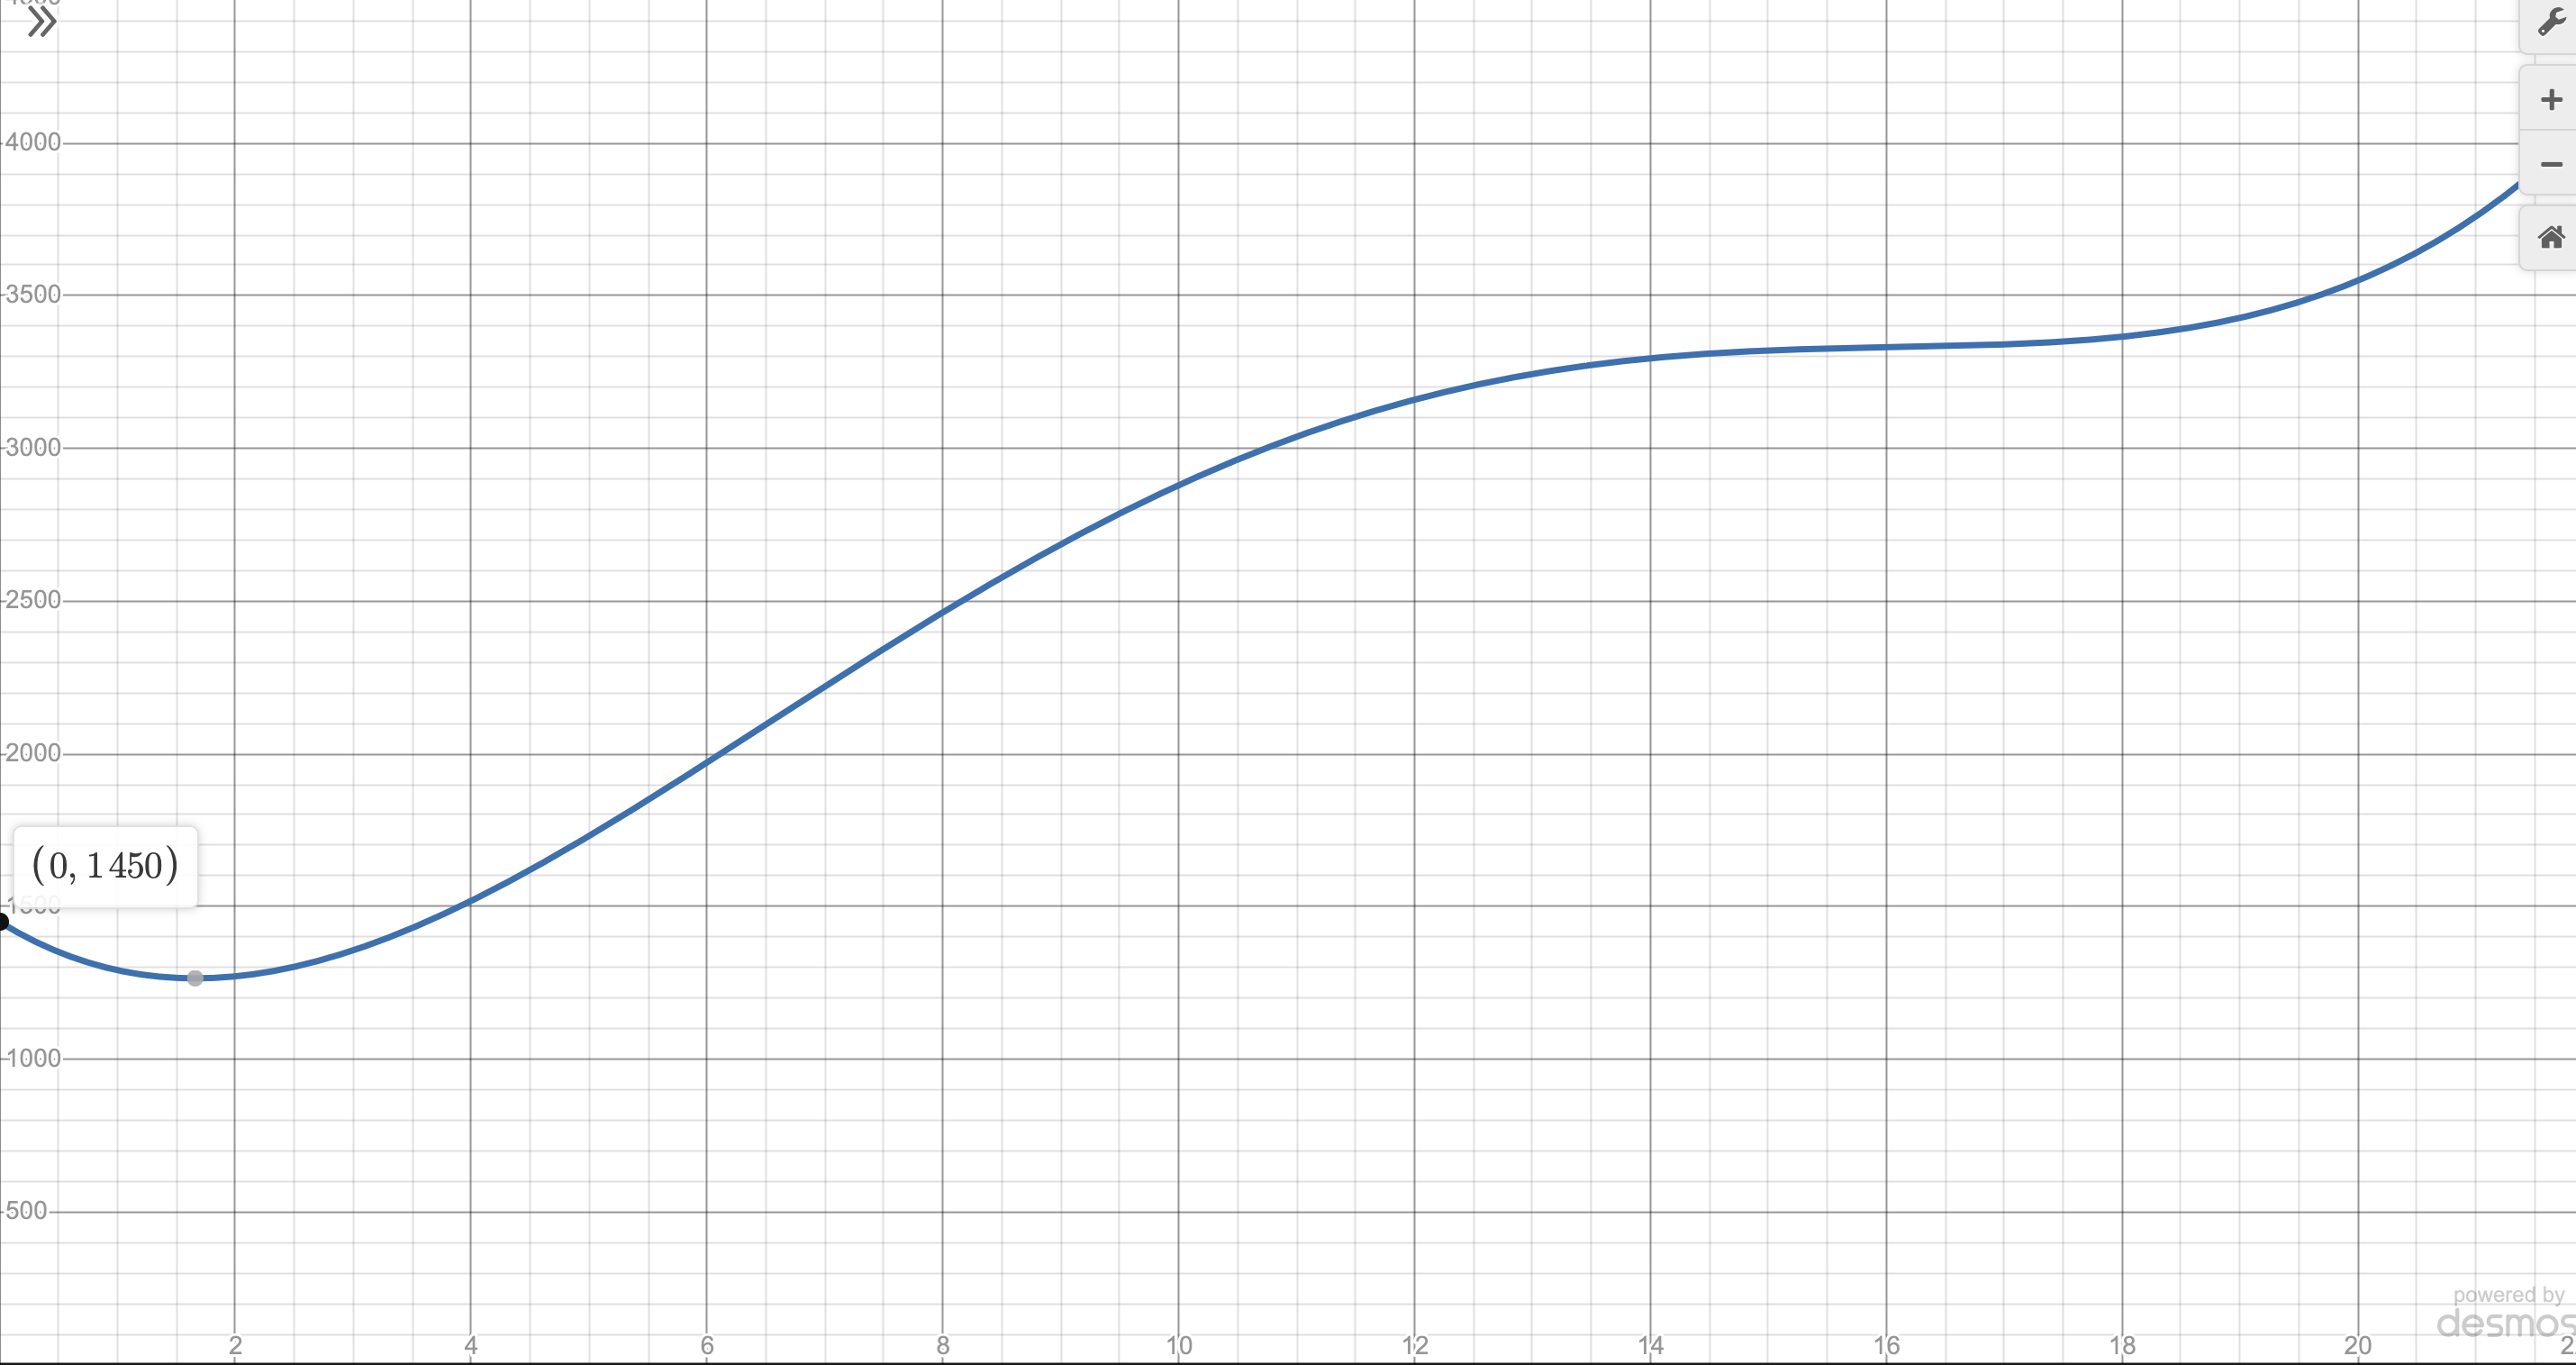
\includegraphics[width = 4in, height = 4in]{2.2picture4}
\newline (c): The given graph gives a value of about $15700$ for the year $2010$ (that is, when $x=30$).
We cannot use this model to predict the number of quarterly periodicals in the year 2010. This is because the year $2010$ is not in the range 
$1980$ to $2002$, meaning the given model does not account for data in that year. In addition, even if we were to say that this could be a very rough 
estimate of the value in $2010$, the amount of Periodicals could change rapidly through the years (for example, due to the rise of the internet), meaning 
this prediction would be at best very rough.

\section*{59}
(a): We are given the two models. From the first model, we can tell that the weight of a 5-day-old Sarus crane chick is $-0.122(5)^3+3.49(5)^2-14.6(5)+136
=135$ and the weight of a 5-day-old hooded crane chick is $-0.115(5)^3+3.71(5)^2-20.6(5)+124=99.375$ meaning the difference in weight is 
$135-99.375=35.625$ grams.\newline
(b):\newline 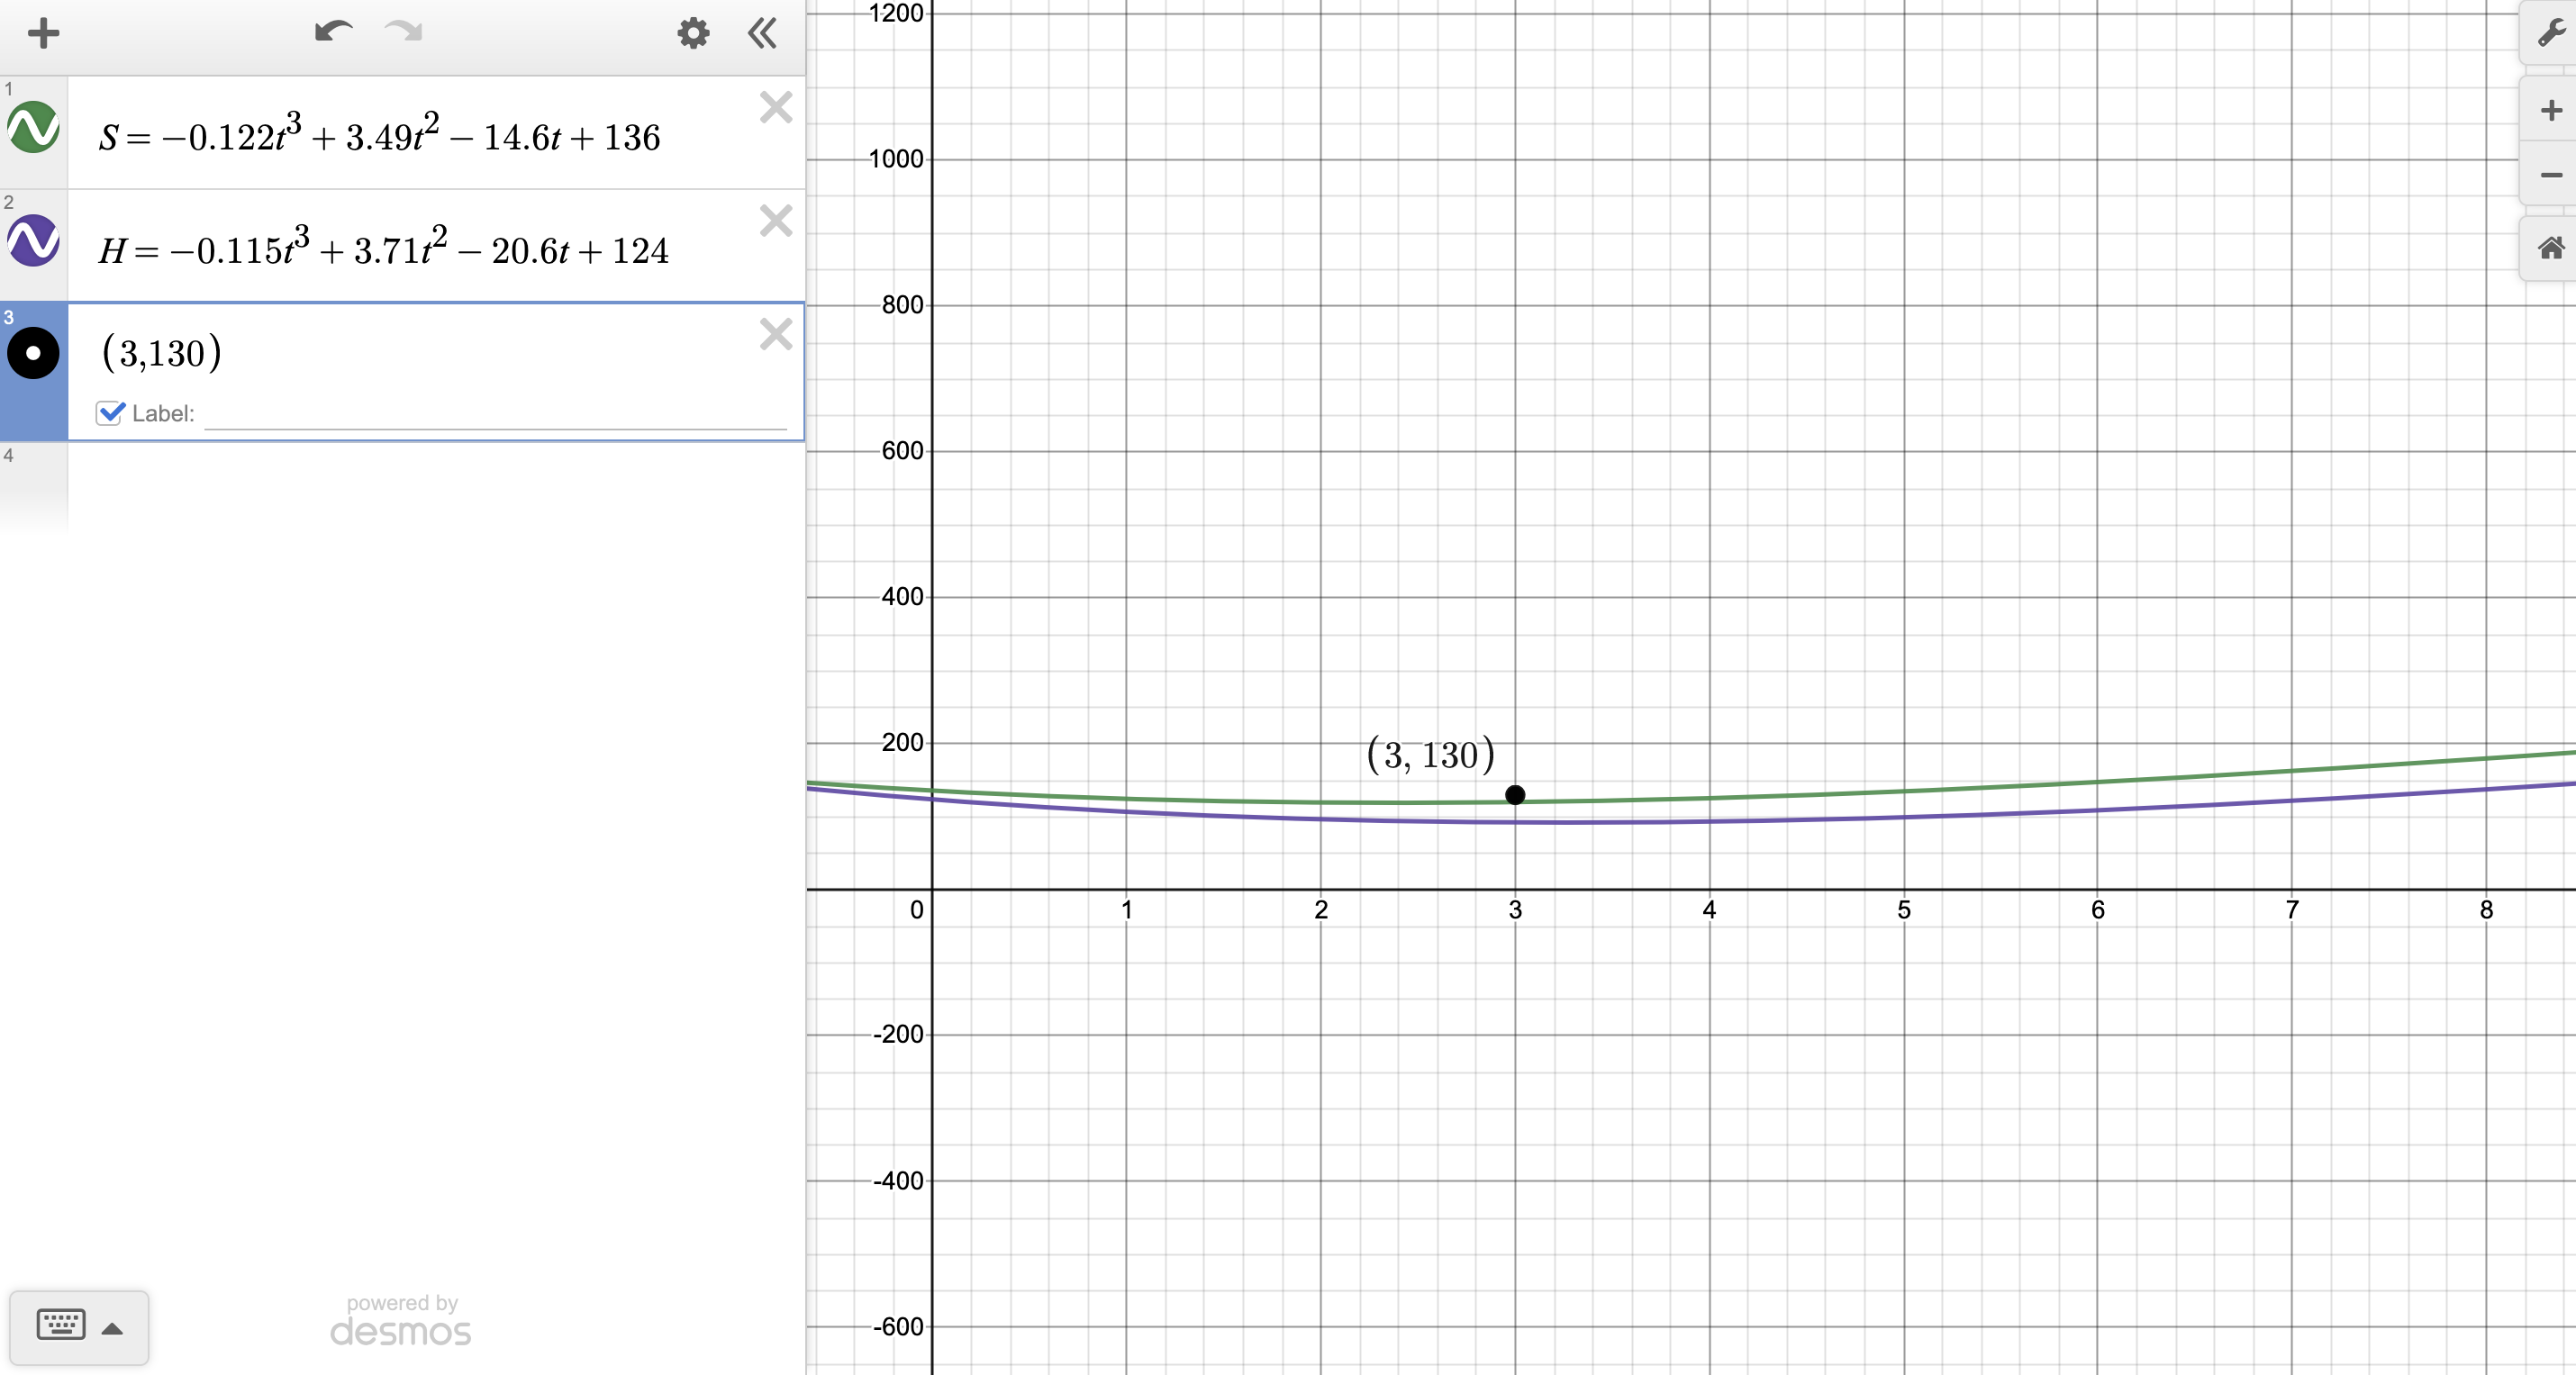
\includegraphics[width = 4in, height = 4in]{2.2picture5}
\newline
(c): From the graph, it can be seen that the point $(3,130)$ is slightly above the green graph, the one representing the Sarus crane chicks. 
Because of this, it is closer to the values found on the green graph, the one for the Sarus chicks, meaning it is most likely a Sarus crane chick.

\section*{60}
(I was not confident with my answer for part (c), so we should go over that)\newline
(a): We are given the fuction $y=0.000304x^3$ where $y$ is measured in pounds and $x$ is measured in inches. If we want to convert this fuction 
to a function where $y$ is measured in kilograms and $x$ is measured in centimeters, we need to multiply $x$ and $y$ by their scale factors in relation 
to centimeters and kilograms, respectively. We are given that $1$ kilogram $\approx 2.20$ pounds and that $1$ centimeter $\approx 0.394$ inches, 
meaning the desired function is $\frac{1}{2.2}y=0.000304(0.394x)^3$ or $y=0.000040906x^3$
\newline (b):\newline 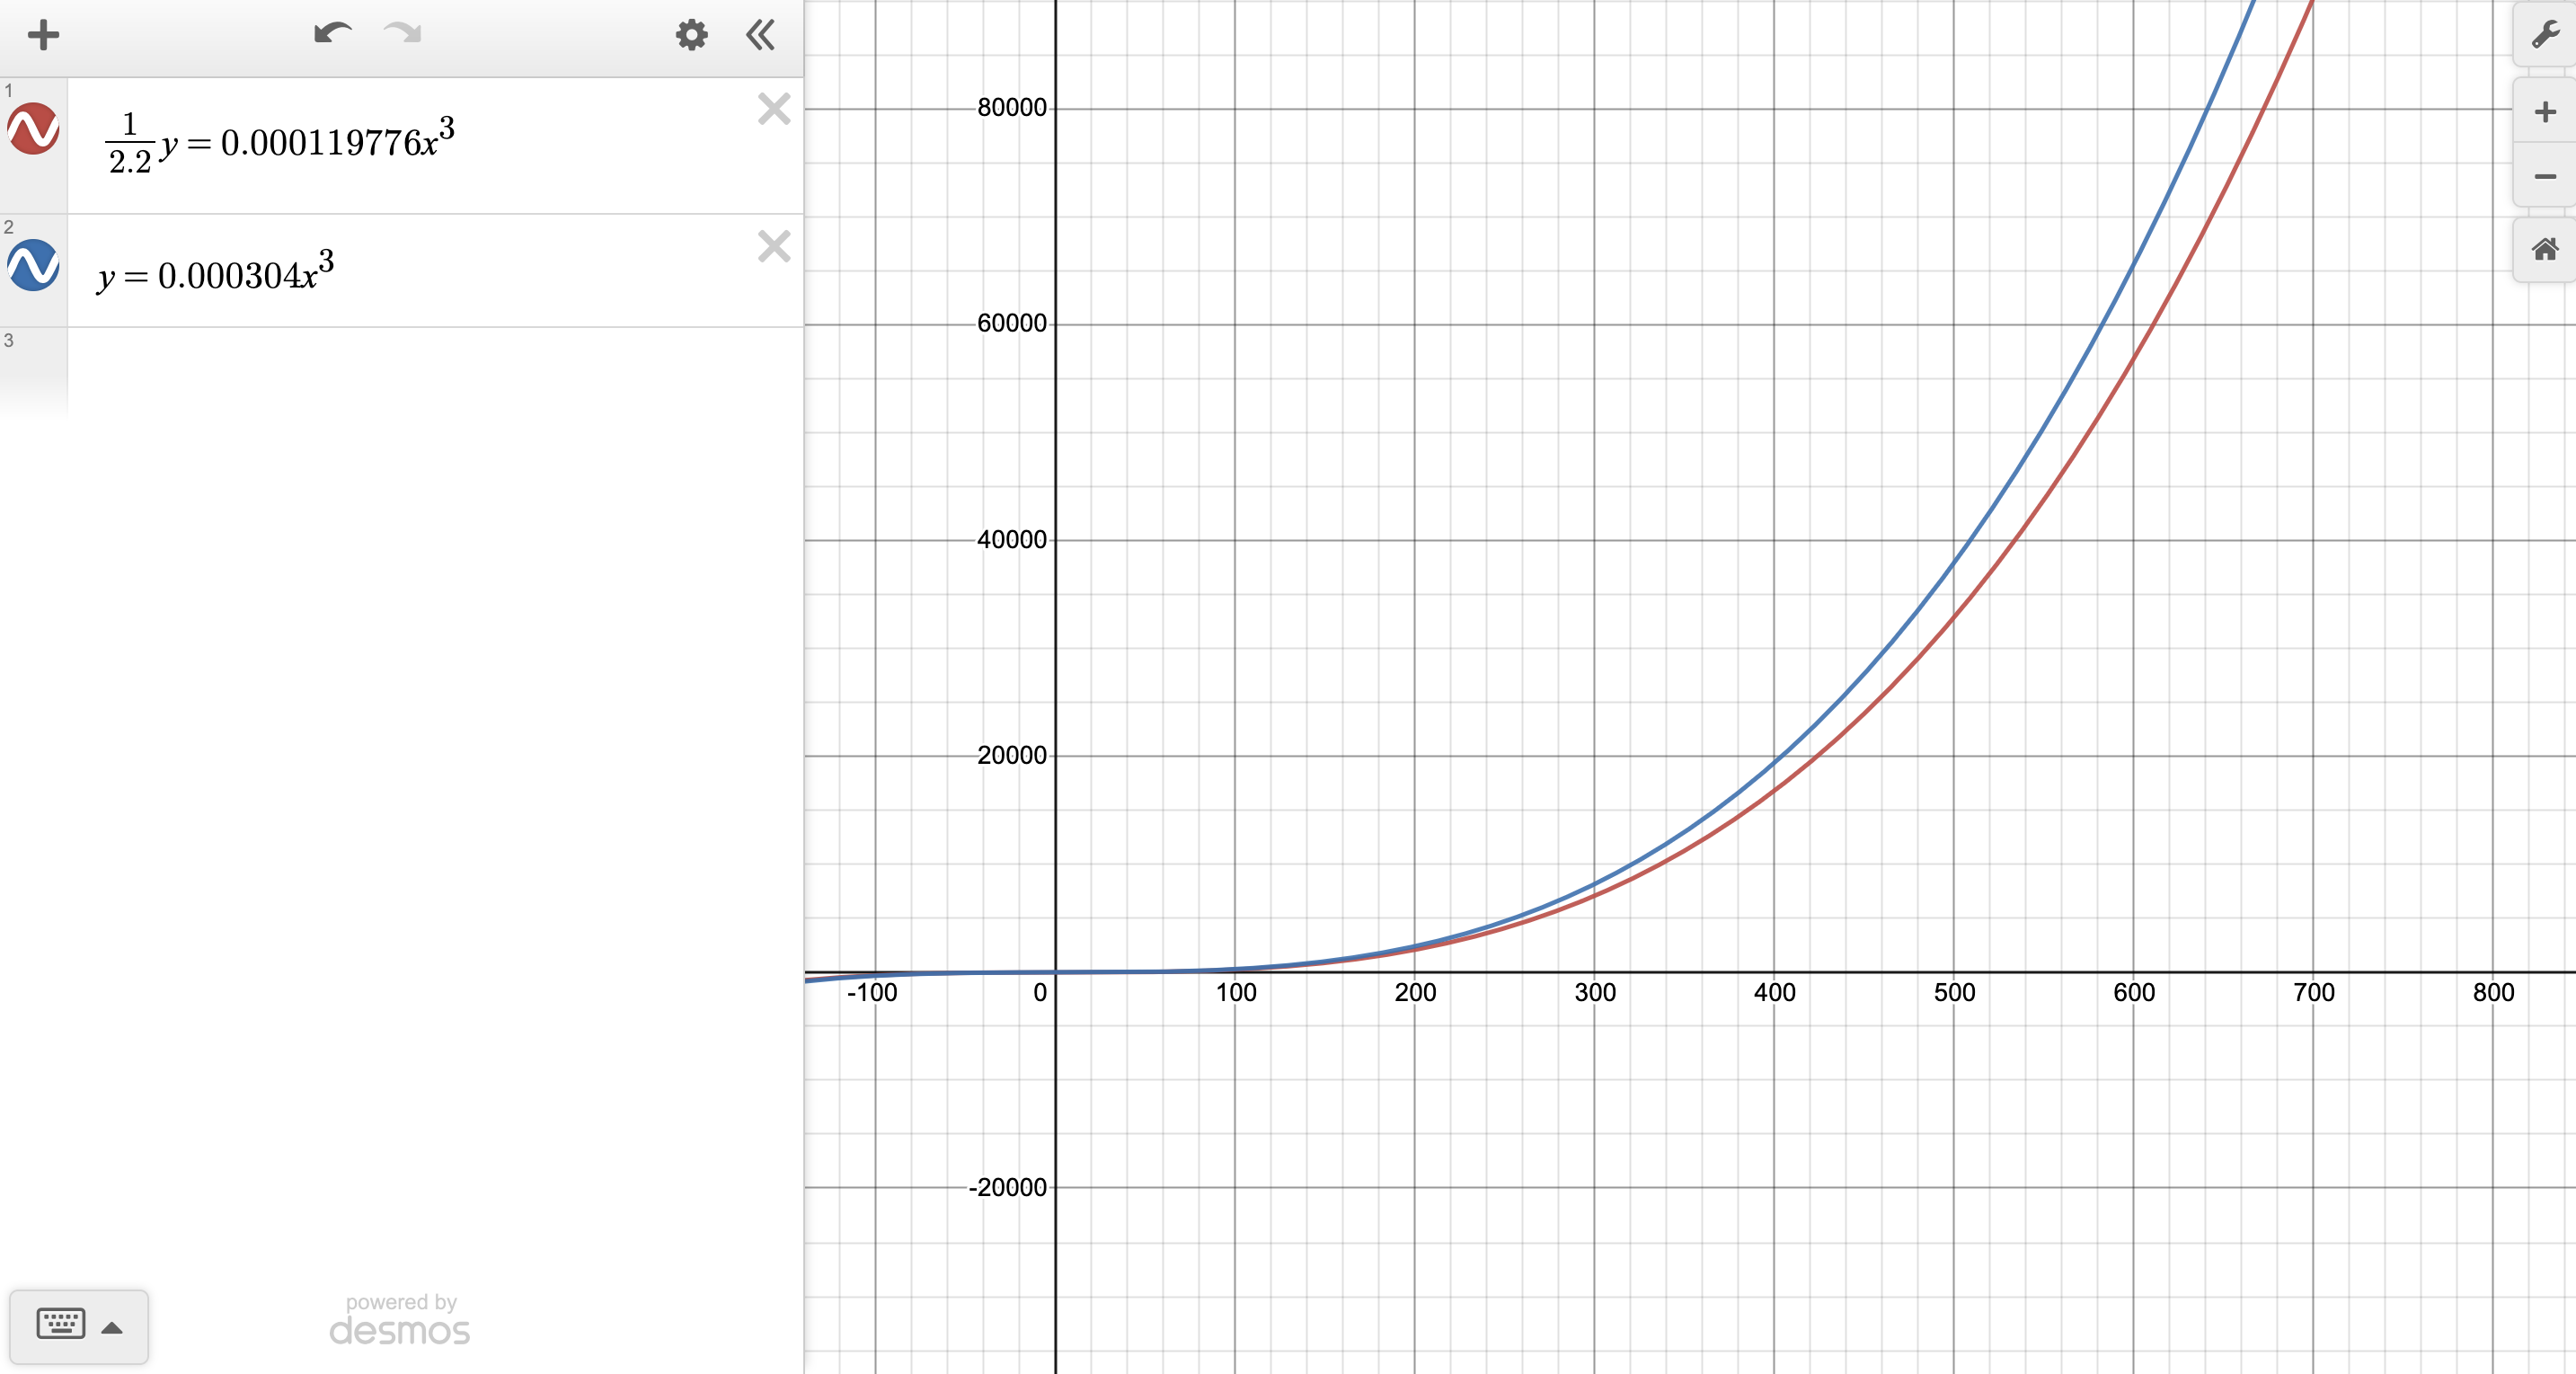
\includegraphics[width = 4in, height = 4in]{2.2picture6}
\newline (c): To go from the original graph to the graph from part (a), we would need to multiply the function $f(x)$ by $0.394\times 2.2\approx 0.8668$
 where $f(x)=0.000304x^3$.
\end{document}


